\documentclass[11pt]{article}
\usepackage{amsmath}
\usepackage{graphicx}
\title{Introduction to Machine Learning}
\author{Your Name}
\date{2024}

\begin{document}

\maketitle

\section{Lecture 4: Unsupervised Learning}

\subsection{Principal Component Analysis (PCA)}

\textbf{Dimension reduction} is used to distill a set of variables into a smaller set of variables that capture the meaningful variation of the original set.
For example, we might take 50 variables and collapse them into 10.
This works very well when a lot of the variables are highly correlated.
For example, in a medical setting, 'heart health' will have multiple measures but we may wish to reduce down to the most meaningful, such as blood pressure.
Dimension reduction is also useful for visualization of data.

\textbf{Principal Component Analysis} is the most useful method for dimension reduction.
Computationally, PCA works by using a subset of the eigenvectors of the data as the new dimensions.
The eigenvectors with the largest eigenvalues serves as the principal components.
We then specify the number of dimensions we want and take the eigenvectors accordingly.

Eigenvectors and eigenvalues are a useful concept from linear algebra, calculated through singular value decomposition. Definining these, an eigenvector for a matrix $A$ has the property such that $Ax = \lambda x$, where $x$ is a vector and $\lambda$ is a scalar.

As an example, consider matrix $A$ as matrix $ \begin{bmatrix}
    1 & 3\\
    3 & 1
\end{bmatrix}$, we could show that the eigenvectors are $ \begin{bmatrix}
    1\\
    1
\end{bmatrix}$ and $ \begin{bmatrix}
    1\\
    -1
\end{bmatrix}$, with eigenvalues $4$ and XXX.

Programmatically, R's 'prcomp' function allows us to get the eigenvectors from data.
We can then use those eigenvectors to transform the data.
The data are rotated, such that they primarily vary across the x-axis.
In practice, the transformation is by taking the coordinates of each point and multiply the $x$ coordinate by the eigenvector to get its 'rotated' coordinate.
We want to have the maximum variance along the x-axis, and this approach allows this.
The rotated data primarily vary along the x-axis, and so we can be in a position to drop the y-axis.
A starting workflow is shown in Figure \ref{fig:PCA_Image1}; a next step from this would be to plot the principal components pairwise, looking for 'gaps' in the pairwise (correlation) plots.
Similarly to EFA, we can use the scree plot, or a cumulative variance plot, to determine the number of components to keep.

\begin{figure}[ht]
    \centering
    \caption{Visualization of PCA workflow.}
    \label{fig:PCA_Image1}
    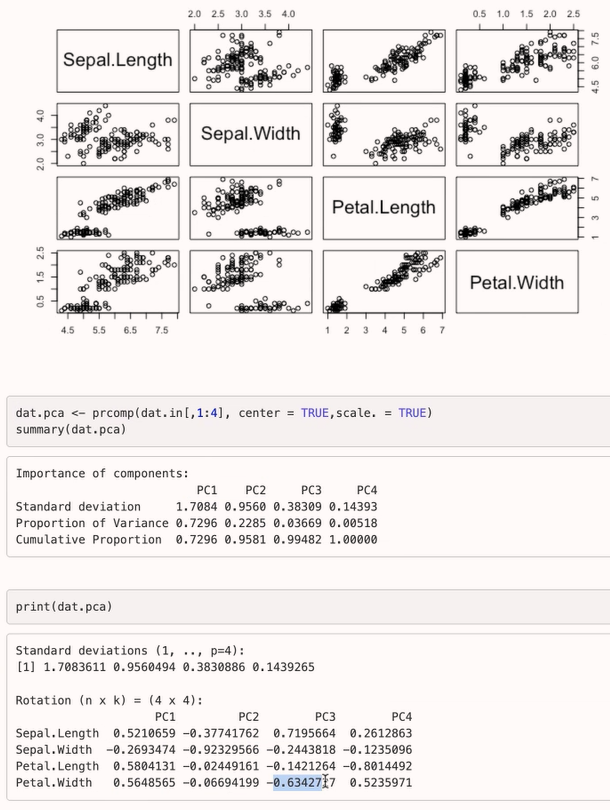
\includegraphics[width=\textwidth]{Images/PCA_Image1.png}
\end{figure}

\subsection{Background on Unsupervised Learning}

Unsupervied learning is used when there is no label to be predicted or estimated.
Clustering is the primary type of unsupervised learning, and the goal of clustering is to divide the data into groups such that the data within a group are more similar to each other than to data in other groups - that is, meaningfully distinct groups. 
The measure of 'similarity' drives the approach taken and results. Some common measures include:

\begin{itemize}
    \item Euclidean distance: Measures the straight-line distance between two points in Euclidean (normal geometric) space.
    \item Hamming distance: measure for two binary strings and averages the number of differences.
    \item Manhattan distance: Also known as L1 distance, it measures the distance between two points by summing the absolute differences of their coordinates.
    \item Cosine similarity: Measures the cosine of the angle between two vectors, often used in text analysis.
    \item Jaccard index: Measures the similarity between two sets by dividing the size of their intersection by the size of their union. It is often used for binary attributes.
\end{itemize}

We also have probabilistic and information theoretic measures.

\subsection{Evaluating Unsupervised Learning Approaches}

\end{document}